\chapter{[SKE] Parametrické modely s (ne)monotónní intenzitou poruch, únavové cyklické zkoušky, příklady použití.}

\begin{define}[Normální rozdělení]
	Mějme $T\sim \NN(\mu, \sigma^2)$ (kde zanedbáme zápornou část, tedy chceme $\mu$ dostatečně daleko od nuly). Platí, že 
	$$ \FR(t)=\frac{\frac{1}{\sigma}\phi\big(\frac{t-\mu}{\sigma}\big)}{1-\Phi\big(\frac{t-\mu}{\sigma}\big)}.$$
	Dále se může použít useknuté normální rozdělení v $t=0$ zleva 
	$\mathcal{TN}(\mu,\sigma^2)$, tedy 
	$$\RT(t)=\frac{\PP(T>t)}{\PP(T>0)}=\frac{1-\Phi\big(\frac{t-\mu}{\sigma}\big)}{1-\Phi\big(\frac{\mu}{\sigma}\big)}.$$
	 Pro $t>0$ je $\FR(t)$ shodná s předešlým případem.
\end{define}

Normální rozdělení se tedy dá použít na modelování třetí fáze opotřebování výrobku.

\begin{define}[Gamma rozdělení]
Mějme $T_i\sim \Exp(\lambda)$. Pak $T:=\sum_{1}^{k}T_j$ je čekací doba na výskyt $k$-té poruchy (třeba pokud máme $k$ náhradních dílů). Tím dostáváme $T\sim\mathrm{Gamma}(k,\lambda)$. $\lambda>0$ nazýváme \textbf{intenzita šoků} a $k>0$ míru rezistence. Víme dále, že $\MTTF=\E T=\frac{k}{\lambda}$. 
\end{define}

\begin{define}[Weibulovo rozdělení]
	Definujeme \textbf{Weibulovo} rozdělení definováno vztahem $\RT(t)=\e{-(\lambda t)^\alpha}$, tedy $f_T(t)=\alpha \lambda^\alpha t^{\alpha-1}\e{-(\lambda t)^\alpha}$. Platí, že
	$$ \FR(t)=\alpha\lambda^\alpha t^{\alpha-1},~\MTTF=\frac{1}{\lambda}\Gamma\big(1+\frac{1}{\lambda}\big),~t_\mathrm{med}=\frac{1}{\lambda}(\ln2)^{1/\alpha}.$$
\end{define}

\begin{theorem}[Reprodukce pro minimum]
	Mějme $(T_i)_{i=1}^n~iid~\Weib(\alpha,\lambda_j)$, $\forall j$. Potom platí, že 
	$$ T_s:=\min(T_i)_{i=1}^n \sim 
	\Weib\big(\alpha,\left\|\boldsymbol{\lambda}\right\|_\alpha\big)\equal{\lambda_j=\lambda}\Weib\big(\alpha,\lambda
	 n^{1/\alpha}\big).$$
\end{theorem}

Toto se velice hodí na sériové systémy, protože systém je vyřazen při pokažení libovolné části systému (třeba zapojení žárovek).

\begin{define}[Lognormální rozdělení]
	Platí, že $T\sim \LN(\mu,\sigma^2)~\Leftrightarrow~\ln 
	T\sim\NN(\mu,\sigma^2)$. Dále platí, že $$\RT(t)=\PP(T>t)=\PP(\ln 
	T>\ln t)=\PP\Big(\frac{\ln T-\mu}{\sigma}>\frac{\ln 
	T-\mu}{\sigma}\Big)=1-\Phi\Big(\frac{\ln T-\mu}{\sigma}\Big),$$ 
	tedy $f_T(t)=-\RT'(t)=¨\frac{1}{\sqrt{2\pi}\sigma 
	t}\e{-\frac{1}{2\sigma^2}(\ln t-\mu)^2}$, vše pro $t>0$.
\end{define}

Dále platí, že $t_\mathrm{med}=\e{\mu}$, $\MTTF=\e{\mu+\frac{\sigma^2}{2}}$, $t_\mathrm{mod}=\e{\mu-\sigma^2}$ a $\D T=\e{2\mu}\big(\e{2\sigma^2}-\e{\sigma^2}\big)$. Pro FR (ponecháno čtenáři) platí, že $\lim\limits_{t\to+\infty}\FR(t)=0$.

Tento model se dá použít jako doba do opravy, nebo u cyklických trhacích zkoušek.

\section{Únavové zkoušky materiálu}
Při těchto zkouškách jde o to, aby se např. vyzkoušel materiál před 
tím, než je použitý na nějaký výrobek. Tento materiál se upne do 
trhacího přístroje a nechá se posílat do materiálu sílu nějakým 
cyklickým způsobem, např. sinusoidní síla $F_s=s\sin(\phi t)$. Při 
různé amplitudě $s$ (stresor) se materiál chová jinak, při nějaké se 
neděje nic, při nějaké se materiál může roztrhnout. Označme $N$ jako 
počet cyklů do rozlomení materiálu. Tato veličina je výrazně propojena 
z časem do poruchy $T=N\cdot\Delta t$. 

Průběh může být třeba i lognormální, při výrobě můžou vzniknout vady a 
ty můžou součástku roztrhnout. Po nějaké době se však všechny tyto 
vady projeví a intenzita poruch začíná klesat (bohužel až k nule, ale 
stačí to k aproximaci).

Fyzikální opodstatnění spočívá v tom, že $Ns^b=c$, kde $b$ a $c$ jsou konstanty, které závisí na daném materiálu (geometrie, složení apod.). Po zlogaritmování dostaneme lineární vztah (k lineární regresi)
$$ \ln N=\ln c-b\ln s + \epsilon, $$
protože $\ln N\sim \NN$.

\begin{figure}[h]
	\centering
	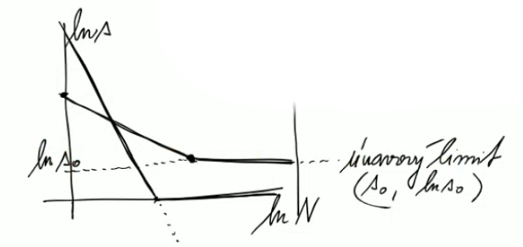
\includegraphics[width=0.4\linewidth]{pictures/Wohler}
	\caption{Wöhlerův diagram. Po dosažení únavového limitu materiál 
	začne pružit. Dále už se regrese nenechá klesnout. Např. gumička s 
	minimální silou bude jen pružit a nepraskne.}
	\label{fig:wohler}
\end{figure}


\begin{define}[Birnbaum-Sanders (BS) rozdělení]
	 Mějme $n$ únavových cyklů se zatížením $s$. Částečné poškození součástky po $i$-tém cyklu nazveme $Z_i$. Předpokládejme, že $Z_1,...,Z_n~id/iid\sim \big(\mu(s),\sigma^2(s)\big)$. Označme celkové poškození jako $W_n=\sumin Z_i$ a kritickou hranici poškození jako $w$ (poté se materiál roztrhne). Platí, že 
	 \begin{align*}
	 \PP(N\leq n)\sim \PP(W_n>w)&=1-\PP\big(\sumin Z_i\leq 
	 w\big)\equal{CLT}1-\PP\Big(\frac{\sumin 
	 Z_i-n\mu}{\sqrt{n}\sigma}\leq 
	 \frac{w-n\mu}{\sqrt{n}\sigma}\Big)=\\&=1-\Phi\Big(\frac{w-n\mu}
	 {\sqrt{n}\sigma}\Big). 
	 \end{align*} 
	 Přejděme nyní k $N\leftrightarrow T$ a $n\leftrightarrow t$. Dostaneme tím 
	 $$ \PP(T\leq 
	 t)=1-\Phi\Big(\frac{w-t\mu}{\sqrt{t}\sigma}\Big)=1-\Phi\Big(\frac{1}{\alpha}\big(\frac{1}{\sqrt{\lambda
	  t}}-\sqrt{\lambda t}\big)\Big), $$ kde 
	 $\alpha=\frac{\sigma}{\sqrt{\mu w}}>0$ a 
	 $\lambda=\frac{\mu}{w}>0$. Potom 
	 $\RT(t)=\Phi\Big(\frac{1}{\alpha}\big(\frac{1}{\sqrt{\lambda 
	 t}}-\sqrt{\lambda t}\big)\Big)$, což je spolehlivost 
	 $\BS(\lambda,\alpha)$ rozdělení. Můžeme také vypočítat 
	 $f_T(t)=C\e{-\frac{1}{2\alpha^2}\big(\sqrt{\lambda 
	 t}-\frac{1}{\sqrt{\lambda t}}\big)^2}$, takže má trochu těžší 
	 chvosty, než normální rozdělení (ale menší, než lognormální 
	 rozdělení). Dále $\E 
	 T=\frac{1}{\lambda}\Big(1+\frac{\alpha^2}{2}\Big)$ a $\D 
	 T=\frac{\alpha^2}{\lambda^2}\Big(1+\frac{5\alpha^2}{4}\Big)$.
\end{define}

% lec 5

\begin{define}[Gompertz-Makehamovo rozdělení]
	Definujeme Gompertz-Makehamovo rozdělení vztahem 
	$$ \FR(t)=\beta+\alpha \e{\gamma t}. $$
\end{define}

\begin{define}[Log-logistické rozdělení]
	Definujeme Log-logistické rozdělení vztahem 
	$$ \RT(t)=\frac{1}{1+(\frac{t}{\sigma})^\beta}.$$

\end{define}

\section{Neparametrické metody}
Mějme nyní $T\sim\FT$, data $\textbf{t}=(t_1,...,t_n)$ a tedy uspořádaný výběr $\big(t_{(1)},...,t_{(n)}\big)$. Z toho můžeme udělat odhady $\overline{t_n}$, $\widehat{t_\mathrm{med}}$, $\hsn$, výběrový koeficient variace $\widehat{\mathrm{CV}}=\frac{s_n}{|\overline{t_n}|}$ a výběrovou disperzi $\widehat{\mathrm{CV}}^2$. Výběrový koeficient variace se dá využít třeba k detekci exponenciálního modelu ($\mathrm{CV}=1$) apod.

Dále můžeme získat empirickou spolehlivostní funkci $R_n(t)$, všechny vlastnosti jako nestrannost, konzistenci, AN apod. se přenáší z distribuční funkce.

Často se ještě používá modifikace empirické spolehlivostní funkce se jménem Crowderův plot, který vynese dvojice $\big\{t_{(j)}, \overline{R_n}\big(t_{(j)}\big)\}_{j=0}^n$, kde $t_{(0)}=0$ a $\overline{R_n}\big(t_{(0)}\big)=1$ a $\overline{R_n}\big(t_{(j)}\big)=\frac{R_n\big(t_{(j)}\big)+R_n\big(t_{(j)-}\big)}{2}$ (funkce připomíná klesající schody, kde skoky jsou nahrazeny prostředním bodem). Použití nalezneme třeba v porovnání $\overline{R_n}$ s Weibulovým rozdělením a můžeme se podívat, jak si dané křivky odpovídají.

Dále se může použít například Weibull Probability Plot. Pokud totiž $T\sim\Weib(\lambda,\alpha)$, pak $\RT(t)=\e{-(\lambda t)^\alpha}$, tedy $\ln\big(-\ln R(t)\big)=\alpha\ln\lambda+\alpha\ln t$. Potom se nabízí udělat Crowderův plot, tedy $\ln t$ oproti $\ln\big(-\ln R(t)\big)$ je přímka, pokud sedí Weibulovský model. Můžeme tedy definovat WPP plot pro data $\textbf{t}$ jako $\big\{\ln t_{(j)},\ln\big(-\ln \overline{R}(t_{(j)})\big)\}_1^n$. Pokud se skutečně ukáže lineární závislost, pak je Weibull dobrý kandidát na spolehlivostní model.

